
\newpage{\ } 
\thispagestyle{empty} 

\chapter{Procesamiento de im\'agenes satelitales}
\lhead{Capítulo 3. \emph{Procesamiento de im\'agenes satelitales}} % This is for the header on each page - perhaps a shortened title
La teledetecci\'on presenta un principio base similar al de la visi\'on, permitiendo mediante una fuente de energ\'ia, un objetivo o escena y un sensor, generar im\'agenes digitales que posibilitan resaltar aquellos elementos dif\'iciles de percibir o ser distinguidos directamente a trav\'es de una imagen normal. A todo esto sum\'andole el comportamiento caracter\'istico que poseen los recursos naturales a sensores espaciales, nos posibilita el empleo amplio de t\'ecnicas de procesamiento de im\'agenes provechosos para el logro de los objetivos en la investigaci\'on. Este capitulo consiste en brindar conceptos espec\'ificos utilizados por la metodolog\'ia, posibilitando comprender la influencia de cada factor en el empleo de im\'agenes satelitales para la estimaci\'on de p\'erdida del contenido de carbono forestal.

\section{Sensores Remotos}
Los sensores remotos nos permiten obtener informaci\'on de la superficie terrestre, soportados en diferentes plataformas (terrestre, \'area y satelital), mediante la captura de energ\'ias reflejadas o radiadas proveniente del sol (sensores pasivos) o del mismo sensor (sensores activos) para luego ser transformadas en productos con diversos y diferentes especificaciones, siendo fotografi\'as \'areas e im\'agenes de sat\'elites los m\'as conocidos.
\subsection{El espectro electromagn\'etico}
A pesar de que las longitudes de ondas son continuas, se establece un serie de bandas donde las radiaciones manifiestan un comportamiento similar organizando las de este modo, en un espectro electromagn\'etico\cite{remote2010abdulrahman}.
Las bandas m\'as empleadas son las siguientes\cite{salinero2002teledeteccion}:
	\begin{itemize}
		\item \textbf{Espectro visible:} (400 nm a 700 nm) se denomina as\'i por tratarse de la \'unica radiaci\'on electromagn\'etica que pueden percibir nuestros ojos, coincidiendo con las longitudes de onda en donde es m\'axima la radiaci\'on solar. Dentro de esta se distinguen tres bandas fundamentales: Azul (400 nm a 500 nm), verde (500 nm a 600 nm) y rojo (600 nm a 700 nm).
		\item \textbf{Infrarrojo pr\'oximo:} (700 nm a 1300 nm) se utiliza para discriminar masas vegetales y concentraciones de humedad.
		\item \textbf{Infrarrojo medio:} (1,3 um a 8 um) en esta franja se entremezclan los procesos de reflexi\'on de la luz solar y de emisi\'on de la superficie terrestre. Se utiliza para estimar contenido de humedad en la vegetaci\'on y los focos de alta temperatura.
		\item \textbf{Infrarrojo lejano o térmico:} (8 um a 14 um) se detecta el calor de la mayor\'ia de las cubiertas terrestres.
		\item \textbf{Microondas:} (a partir de 1 um) de gran inter\'es por ser un tipo de energ\'ia transparente a la cubierta nubosa.
	\end{itemize}

\subsection{Firmas espectrales}
Las firmas espectrales consisten en la represntaci\'on de energ\'ia reflejada con relaci\'on a las longitudes de ondas, consideradas sin el efecto atmosf\'erico y medida en condiciones ideales del \'angulo incidente. Ayudan a identificar los objetos en la superficie terrestre debido a que cada uno presenta una respuesta espectral \'unica\cite{sivakumar2004satellite}.\\~\\
En la siguiente figura se observa como cada objeto difiere de los dem\'as en sus firmas espectrales:

\begin{figure}[!hbtp]
	\centering
	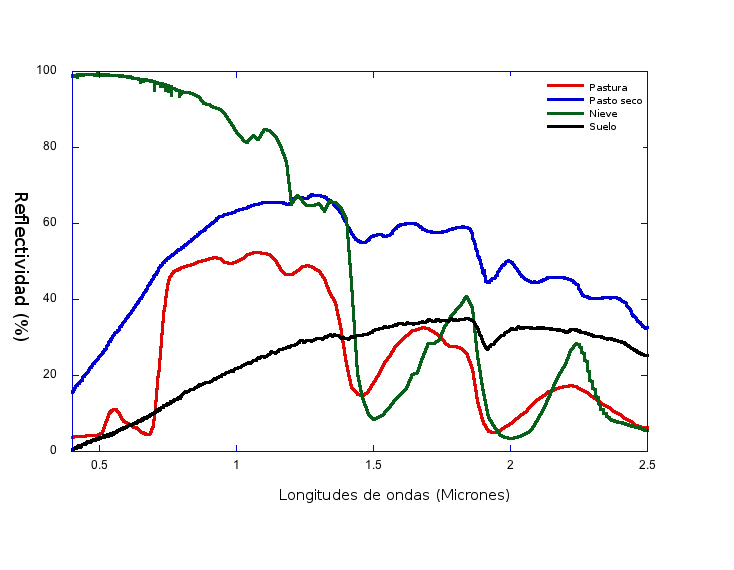
\includegraphics[width=0.9	\textwidth]{./Figures/cap3/firmaEspectral.jpg}
	\caption{Firmas espectrales de diferentes coberturas.}
	\label{fig:firmaEspectral}
\end{figure}

\subsection{Resoluciones de un sensor}

Se define a la resoluci\'on de un sensor como el menor cambio en la magnitud de entrada que puede ser apreciada en la magnitud de salida. El concepto de resoluci\'on implica al menos cuatro manifestaciones \cite{peralta2013analisis}: 
	\begin{itemize}
		
		\item \textbf{Resolución espacial:} Es el tamaño que representa en el terreno una unidad de pixel de la imagen. Tiene mucha importancia en la interpretaci\'on pues marca el nivel de detalle que ofrece, cuanto menor sea el tama\~{n}o del pixel, menor ser\'a tambi\'en la probabilidad de que corresponda a un compuesto de dos o m\'as \'areas fronterizas.
		\begin{figure}[H]
			\centering
			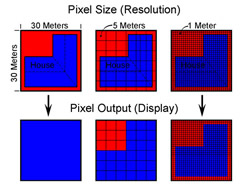
\includegraphics[width=0.4	\textwidth]{./Figures/cap3/espatialRes.jpg}
			\caption{Resoluci\'on espacial.}
			\label{fig:espatialRes}
		\end{figure}
			\item \textbf{Resoluci\'on espectral:} Indica el n\'umero y anchura de las bandas espectrales que puede discriminar el sensor. Un sensor ser\'a tanto m\'as id\'oneo cuanto mayor n\'umero de bandas proporcione, ya que facilita la caracterizaci\'on espectral de las distintas cubiertas.
				\begin{figure}[H]
					\centering
					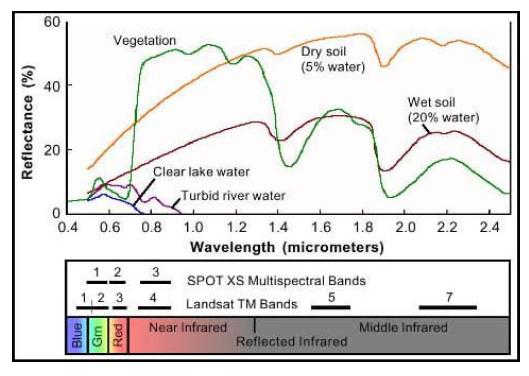
\includegraphics[width=0.6	\textwidth]{./Figures/cap3/resolucionespectral.jpg}
					\caption{Resoluci\'on espectral igual a 3 para el sensor SPOT y 7 en el sensor Landsat.}
					\label{fig:espectralRes}
				\end{figure}
		\item \textbf{Resoluci\'on radiom\'etrica:} Es la sensibilidad del sensor para detectar variaciones en la cantidad de energ\'ia espectral recibida. La sensibilidad se expresa en bits e indica el n\'umero de los distintos niveles radiom\'etricos $ r $ que puede detectar un sensor.
		\nomenclature[10]{$ r $}{Bits o Niveles radiom\'etricos de la imagen satelital.}	
						\begin{figure}[H]
							\centering
							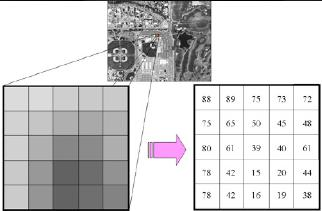
\includegraphics[width=0.6	\textwidth]{./Figures/cap3/resolucionradiometrica.jpg}
							\caption{Resoluci\'on radiom\'etrica de 8 bits (0 a 255 niveles digitales).}
							\label{fig:radioRes}
						\end{figure}
		\item \textbf{Resoluci\'on temporal:} Este tipo de resoluci\'on se refiere al intervalo de tiempo entre muestras sucesivas de la misma zona de la cobertura terrestre. El ciclo de cobertura est\'a en funció\'on de las caracter\'isticas orbitales de la plataforma, su velocidad, el ancho de barrido del sensor y las caracter\'isticas de construcci\'on del sistema.
			\begin{figure}[H]
					\centering
					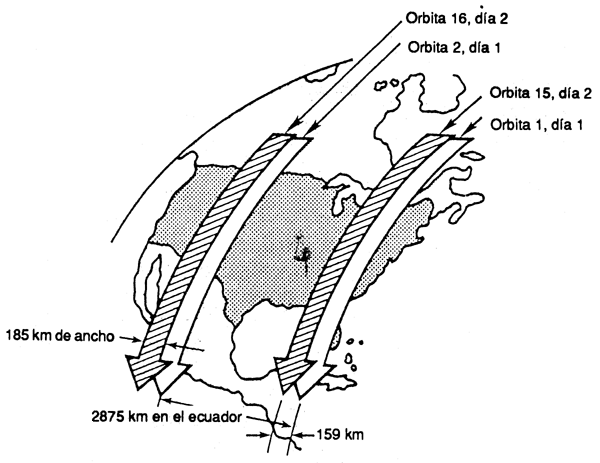
\includegraphics[width=0.6	\textwidth]{./Figures/cap3/temporalRes.png}
					\caption{Resoluci\'on temporal de 16 d\'ias.}
					\label{fig:temporaRes}
				\end{figure}
		

		
	\end{itemize}

\section{Im\'agenes satelitales}
%Una imagen satelital o imagen de sat\'elite $ S $ se puede definir como la representaci\'on visual de la informaci\'on capturada por un sensor montado en un sat\'elite artificial. Est\'an organizados en un arreglo matricial bidimensional $ l \times c $ de elementos llamados p\'ixeles, donde cada p\'ixel representa un \'area de superficie sobre la tierra con un valor de intensidad o nivel digital $ f(x,y) $, dentro del dominio $ D=[0,2^{r}] $, y una ubicación en la imagen  $(x,y)$, tambi\'en son conocidas como im\'agenes r\'aster \cite{acosta2003experiencia}. 
%		\nomenclature[11]{$ S $}{Imagen satelital.}	
%\begin{equation}
%\label{eq:imagenDigital}
%f(x,y)=\begin{bmatrix}
%f(0,0) &f(0,1)  & \cdots & f(0,c-1) \\ 
%f(1,0) & f(1,1) & \cdots  & f(1,c-1)\\ 
%\vdots & \vdots & & \vdots \\ 
%f(l-1,0) & f(l-1,1)  &\cdots  & f(l-1,c-1)
%\end{bmatrix}
%\end{equation}
Una imagen satelital se puede definir como la representaci\'on visual de la informaci\'on capturada por un sensor montado en un sat\'elite artificial \cite{acosta2003experiencia}. \\~\\
Sea $ \mathbb{Z} $ un conjunto de enteros. Una imagen satelital es una funci\'on $ f:\mathbb{Z}^{3} \longrightarrow [0,....,2^{r}) $. Cada $ (x,y,i) $ se los conoce como coordenadas espaciales de la banda $ i $, donde $ i \in [1,k] $, siendo $ k $ el numero de bandas y $ r $ la resoluci\'on radiom\'etrica en la imagen. Las im\'agenes satelitales son conocidos tambi\'en como raster.
  \begin{figure}[H]
  	\centering
  	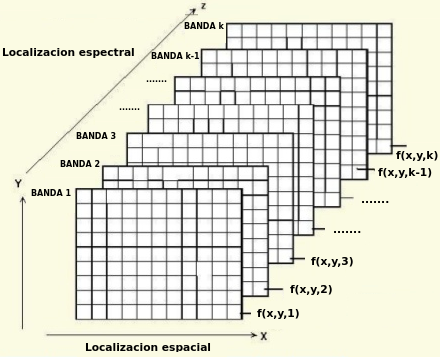
\includegraphics[width=0.8	\textwidth]{./Figures/cap3/imagen_satelital.png}
  	\caption{Imagen satelital.}
  	\label{fig:imagenMultiespectral}
  \end{figure}
La ilustraci\'on \ref{fig:imagenMultiespectral} nos muestra los ejes de coordenadas espaciales $ x $ e $ y $ para cada plano que representan las bandas, pudiendo acceder a valor de la intensidad o nivel digital mediante la funci\'on $ f(x,y,i) $.


\subsection{Histogramas}
El histograma es una representaci\'on gr\'afica \'util de la informaci\'on contenida por las im\'agenes obtenidas a trav\'es de la percepci\'on remota. Los analistas, a menudo despliegan el histograma ya que proporciona una apreciaci\'on de la calidad de los datos que presenta una imagen. Por ejemplo si el contraste es bajo o muy alto (histogramas estrechos y amplios); si son multimodales responden a distintos tipos de coberturas detectadas (agua, humedales, tipos de vegetaci\'on, etc.), si el histograma se encuentra desplazado hacia la izquierda, la imagen tendr\'a una tonalidad oscura y si esta desplazada hacia la derecha tendr\'a una tonalidad mas clara; entre otras interpretaciones.

\subsection{Combinaci\'on de bandas}
Las im\'agenes satelitales suelen ser multiespectrales, es decir que son registradas simult\'aneamente en varias regiones del espectro electromagn\'etico (Bandas). Estas im\'agenes pueden ser estudiadas individualmente en escalas de grises o en im\'agenes coloreadas obtenidas a partir de las primeras. Las im\'agenes coloreadas se generan seg\'un el modelo de color RGB ( Red, Green, Blue). Este hace referencia a la composici\'on del color en t\'erminos de la intensidad de los colores primarios con los que se forma: el rojo, el verde y el azul. Es un modelo de color basado en la s\'intesis aditiva, es decir basado en la mezcla por adici\'on de dichos primarios\cite{teledet2015Combi}.
Mediante el estudio en cada banda, y la combinaci\'on de ellas, es posible resaltar variaciones de color, tonalidad, textura de las rocas, etc. A continuaci\'on se describe algunas combinaciones posibles con im\'agenes Landsat para la identificacion visual de aspectos terrestres\cite{lillesand2014remote}:
	\begin{itemize}
		\item \textbf{Bandas 3,2,1 (RGB):} Es una imagen de color natural. Refleja el \'area tal como la observa el ojo humano en una fotograf\'ia a\'erea a color.
		\item  \textbf{Bandas 7,4,2 (RGB):} Permite discriminar los tipos de rocas. Ayuda en la interpretaci\'on estructural de los complejos intrusivos asociados a los patrones volcano - tect\'onicos.
		\item  \textbf{Bandas 5,4,2 (RGB):} Es una imagen que no refleja los patrones en colores naturales (falso color), por lo tanto las carreteras pueden ser rojas, el agua amarilla y la vegetaci\'on azul.
		\item \textbf{Bandas 7,3,1 (RGB):} Ayuda a diferenciar tipos de rocas, definir anomal\'ias de color que generalmente son de color amarillo claro algo verdoso, la vegetaci\'on es verde oscuro a negro, los r\'ios son negros y con algunas coloraciones azules a celestes.		
	\end{itemize}
 
  \begin{figure}[H]
  	\centering
  	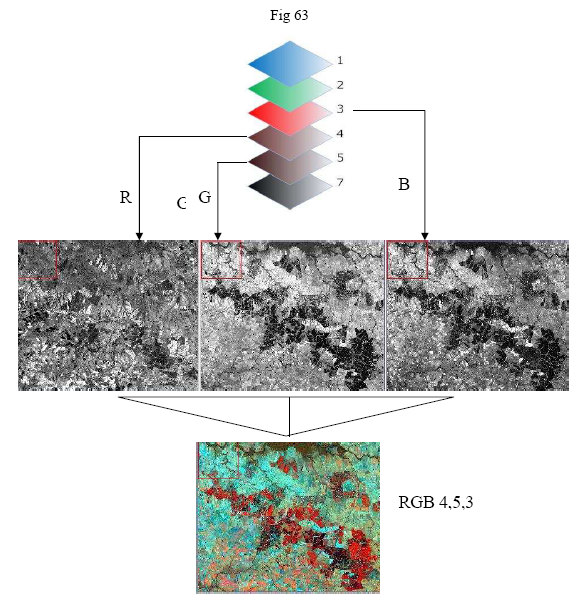
\includegraphics[width=0.8	\textwidth]{./Figures/cap3/combinacionColor.jpg}
  	\caption{Combinaci\'on de bandas espectrales a trav\'es de los canales RGB.}
  	\label{fig:combinacionColor}
  \end{figure}

 
\section{\'Indices de vegetaci\'on}
Los \'indices de vegetaci\'on son transformaciones que implican efectuar una combinaci\'on matem\'atica, entre los niveles digitales almacenados en dos o m\'as bandas espectrales de la misma imagen, teniendo en cuenta el comportamiento radiom\'etrico de la vegetaci\'on vigorosa para la elecci\'on de bandas\cite{speranza2005potencialidad}. \\~\\
El estudio de las cubiertas vegetales mediante la teledetecci\'on se aborda tradicionalmente mediante la utilización de los denominados “índices de vegetaci\'on”, el índice de vegetaci\'on m\'as utilizado es el NDVI (\'Indice de vegetaci\'on diferencial normalizada)\cite{sader2000estimacion}.

\subsection{\'Indice de vegetaci\'on diferencial normalizada}\label{subsec:ndvi}
Es un \'indice usado para estimar la cantidad, calidad y desarrollo de la vegetaci\'on, por medio de sensores remotos instalados com\'unmente desde la plataforma espaciales, es decir mide las condiciones de vigor vegetal de la planta, principalmente su contenido en clorofila\cite{salinero2002teledeteccion}. El objetivo del NDVI es la reducci\'on de m\'ultiples bandas a una sola, condensando la informaci\'on m\'as importante, en este caso la vegetaci\'on.\\~\\
Chuvieco\cite{salinero2002teledeteccion} menciona que la principal ventaja del NDVI es su f\'acil interpretaci\'on, ya que sus
valores var\'ian entre -1 y +1 permitiendo conocer el estado de vigor vegetal en grandes superficies, detectando fen\'omenos de amplio rango.\\~\\
Se calcula extrayendo de las bandas correspondientes al rojo $B_{R}$ e infrarrojo pr\'oximo $B_{IRc}$ seg\'un la siguiente expresi\'on:
	\begin{equation}
	\label{e:ndvi}
	NDVI=\dfrac{B_{IRc}-B_{R}}{B_{IRc}+B_{R}}
	\end{equation}
	\nomenclature[10]{$NDVI$}{Imagen con el \'indice de vegetaci\'on diferencial normalizada calculada.}
	\nomenclature[11]{$B_{IRc}$}{Imagen que representa a la banda infrarroja cercana.}
	\nomenclature[12]{$B_{R}$}{Imagen que representa a la banda roja.}
Las plantas muestran un fuerte pico de absorci\'on causados por los pigmentos fotosint\'eticos en longitudes de onda cercanas a los 700 micrones, hecho que contrasta con una fuerte reflexi\'on de las longitudes de onda del infrarrojo cercano. Por su parte, los suelos desnudos se caracterizan por un incremento suavemente monot\'onico de la reflectancia, a medida que aumenta la longitud de onda.

\section{An\'alisis Multitemporal}
B\'asicamente el an\'alisis multitemporal consiste en el estudio de zonas determinadas mediante tomas hechas en diferentes tiempos, Chuvieco \cite{salinero2002teledeteccion} resalta que el factor temporal puede abordarse con un doble objetivo: por un lado reconstruir la variaci\'on estacional de la zona y por otra parte la detecci\'on de cambios, esta \'ultima se enfoca a detectar cambios entre dos o m\'as
fechas alejadas en el tiempo, estudia el dinamismo temporal de una determinada zona, como por ejemplo: el crecimiento urbano, transformaciones agrícolas, entre otras.\\~\\
Sea uno u otro el enfoque aplicado al estudio multitemporal, resulta preciso abordar previamente una serie de tratamientos sobre las im\'agenes satelitales de cara a garantizar su comparabilidad, ya que existen factores, naturales o las del sensor, que influye desde la captura de informaci\'on hasta su transformaci\'on final a niveles digitales que podr\'ian afectar el an\'alisis.


\section{Correciones a las im\'agenes de sat\'elites}
Una imagen de sat\'elite est\'a sometida a una serie de interferencias que hacen que la informaci\'on que quiere obtenerse aparezca perturbada por una serie de errores:
	\begin{itemize}
		\item Fallos en los sensores, generan pixeles incorrectos.
		\item Alteraciones en el movimiento del sat\'elite y el mecanismo de captaci\'on e los sensores, generan
		distorsiones en la imagen global.
		\item Interferencia de la atm\'osfera, alteran de forma sistem\'atica los valores de los pixeles.
	\end{itemize}


\subsection{Correccci\'on geom\'etrica}\label{sec:corrGeometrica}
Una imagen de sat\'elite, al igual que las fotograf\'ias a\'ereas, no proporciona informaci\'on georreferenciada; cada pixel se ubica en un sistema de coordenadas arbitrario de tipo fila-columna como los que manejan los programas de tratamiento digital de im\'agenes.\\~\\
El proceso consiste en dar a cada pixel su localizaci\'on en un sistema de coordenadas estandard (UTM, lambert, coordenadas geogr\'aficas) para poder, de este modo, combinar la imagen de sat\'elite con otro tipo de capas en un entorno SIG. Mediante esto, se obtiene una nueva capa en la que cada columna corresponde con un valor de longitud y cada fila con un valor de latitud. En caso de que la imagen no hubiese sufrido ningún tipo de distorsi\'on, el procedimiento ser\'ia bastante sencillo, sin embargo una imagen puede sufrir diversos tipos de distorsiones.\\~\\
Es necesario localizar puntos comunes de la imagen con puntos de referencias, como tarea incial para la correcci\'on geom\'etrica, de manera a poder realizar una interpolaci\'on espacial y de los valores radiom\'etricos\cite{deniseCultivos}.

\subsubsection{Interpolaci\'on espacial}
Consiste en la determinaci\'on de la relaci\'on geom\'etrica entre las coordenadas del pixel de la imagen a corregir y las coordenadas correspondientes. Utilizando los puntos comunes localizados, se plantea una ecuaci\'on de transformaci\'on mediante la cual se obtiene la posici\'on de los pixeles en la imagen de salida, ilustrada en la figura \ref{fig:intEspacial}. Este proceso tambi\'en es conocido como Georreferenciaci\'on. El m\'etodo mas utilizado para la transformaci\'on es el de ecuaciones polin\'omicas. 
    \begin{figure}[H]
    	\centering
    	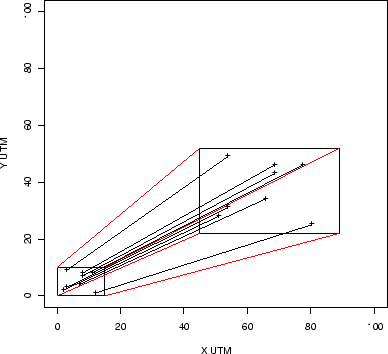
\includegraphics[width=0.9	\textwidth]{./Figures/cap3/inter_spacial.png}
    	\caption{Localizaci\'on de puntos comunes y puntos de referencia.}
    	\label{fig:intEspacial}
    \end{figure}
 
 La transformaci\'on puede expresarse de la siguiente manera:
	\begin{equation}
	x^{,}_{i} = \sum_{j=0}^{g} \sum_{k=0}^{g-j} a_{ij}x^{j}_{i}y^{k}_{i}
	\end{equation} 
		\begin{equation}
		y^{,}_{i} = \sum_{j=0}^{g} \sum_{k=0}^{g-j} b_{ij}x^{j}_{i}y^{k}_{i}
		\end{equation} 

\nomenclature[13]{$ (x,y) $}{Representa las coordenadas de la imagen de entrada.}	
\nomenclature[13]{$ g $}{ Grado del polinomio de ajuste.}
\nomenclature[13]{$ i $}{ Banda de la imagen satelital.}


Donde $ x^{,}_{i} $ e $ y^{,}_{i} $ indica la coordenada en la imagen corregida, $ i $ representa la banda de la imagen, $ x_{i} $ y $ y_{i} $ representan las coordenadas de la imagen de entrada. El superindice $ g $ indica el grado del polinomio de ajuste, $ a_{i} $ y $ b_{i} $ los coeficientes del polinomio. Siendo la ecuaci\'on lineal las mas simple:
	\begin{equation}
	x^{,}_{i} = a_{0}+a_{1}x_{i}+a_{2}y_{i}
	\end{equation} 
		\begin{equation}
		y^{,}_{i} = b_{0}+b_{1}x_{i}+b_{2}y_{i}
		\end{equation} 
		\nomenclature[14]{$ (x^{,},y^{,}) $}{Coordenadas de la imagen transformada.}
En distorsiones moderadas o en un \'area reducida, se utilizan transformaciones de primer orden, pudiendo corregir efectos de translaci\'on en $ x^{,}_{i} $ e $ y^{,}_{i} $, cambios de escala y rotaci\'on.
En distorsiones m\'as importantes o en \'areas extensas, es necesario una transfomaci\'on de segundo orden. Este tipo de transformaci\'on agregan a diferencia del primer orden, correcciones a deformaciones locales.
    \begin{figure}[H]
    	\centering
    	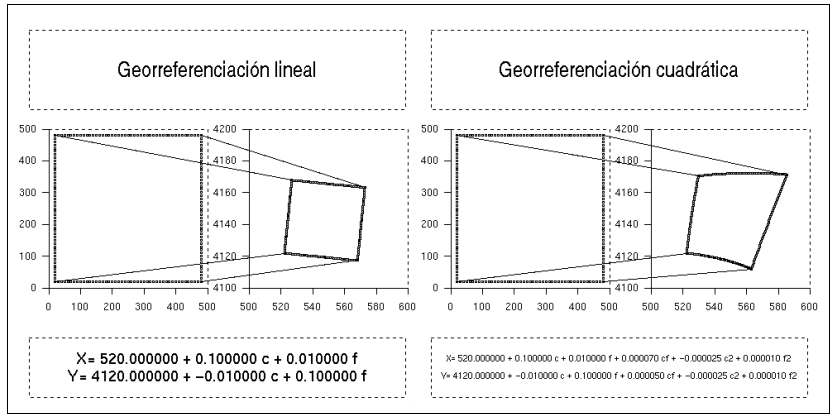
\includegraphics[width=0.9	\textwidth]{./Figures/cap3/ecuacPolinomica.png}
    	\caption{Interpolaci\'on espacial con polinomios de primer y segundo orden.}
    	\label{fig:intPolEcua}
    \end{figure}
 Para calcular la calidad en la interpolaci\'on espacial y los puntos de control seleccionados, se utiliza el error cuadrático medio (RMS), que consiste en la diferencia entre la coordenada re-transformada deseada para un punto de control y la coordenada real obtenida como salida.

 \begin{equation}
 RMS_{error(i)} = \sqrt{(x_{i}^{'}-x_{i})^{2}+(y_{i}^{'}-y_{i})^{2}}
 \end{equation} 
 		\nomenclature[15]{$ RMS_{error(i)} $}{Error cuadr\'atico de la banda $ i $.}
 
 Donde $ x_{i} $ e $ y_{i} $ son las coordenadas de entrada.
 
     \begin{figure}[H]
     	\centering
     	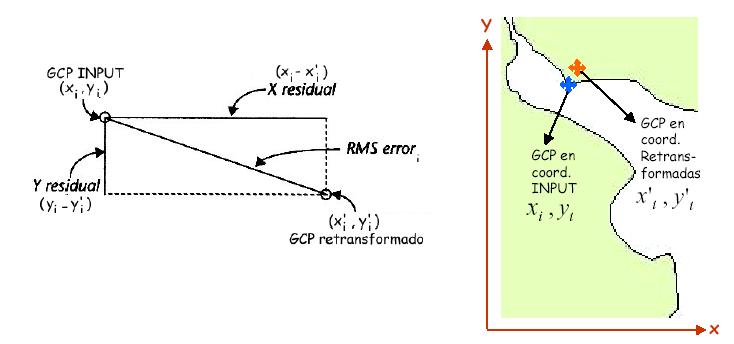
\includegraphics[width=0.9	\textwidth]{./Figures/cap4/rms.png}
     	\caption{Error RMS.}
     	\label{fig:rms}
     \end{figure}



\subsubsection{Interpolaci\'on de los valores radiom\'etricos}
La Interpolaci\'on de los valores radiom\'etricos es el traslado del nivel digital perteneciente a la imagen original, a la imagen corregida. Lo que se pretende es crear una imagen que se corresponda con estas coordenadas, por lo tanto, resulta necesario trasvasar de alguna forma, los niveles digital originales a su nueva posici\'on. Pudi\'endose ser abordada por tres m\'etodos diferentes:
	\begin{itemize}
		\item \textbf{Vecino m\'as pr\'oximo:} situ\'a en cada celda de la imagen corregida el nivel digital $ (Nd) $ del pixel m\'as cercano en la imagen original. Constituye la soluci\'on m\'as r\'apida y la que supone menor transformaci\'on en los niveles digitales originales. Su principal inconveniente es que produce una distorsi\'on en rasgos lineales en la imagen(fracturas, carreteras, caminos), que pueden aparecer en la corregida como lineales quebradas. Algebraicamente puede ser expresado:
		
\begin{equation}
	f(x^{,},y^{,}) = \begin{cases}
		f(x,y) & \text{si }\Delta x < 0.5 \text{ y } \Delta y < 0.5\\
		f(x+1,y) & \text{si } \Delta x \geq 0.5 \text{ y } \Delta y < 0.5\\
		f(x,y+1) & \text{si } \Delta x < 0.5 \text{ y } \Delta y \geq 0.5\\
		f(x+1,y+1) & \text{si } \Delta x \geq 0.5 \text{ y } \Delta y \geq 0.5
	\end{cases}
\end{equation}	

\begin{equation}
	\Delta x = x^{,}-x
\end{equation}	
\begin{equation}
	\Delta y = y^{,}-y
\end{equation}	
\nomenclature[16]{$ f(x,y) $}{ Funci\'on que obtiene el nivel digital en la imagen original.}
\nomenclature[17]{$ f(x^{,},y^{,}) $}{ Funci\'on que obtiene el nivel digital en la imagen corregida.}

		Donde $ f(x,y) $ obtiene el nivel digital de la imagen original, $ f(x^{,},y^{,}) $ el nivel digital de la imagen corregida. En la ilustraci\'on \ref{fig:vecinoMasCercano2} se observa el procedimiento realizado.
				    \begin{figure}[H]
				    	\centering
				    	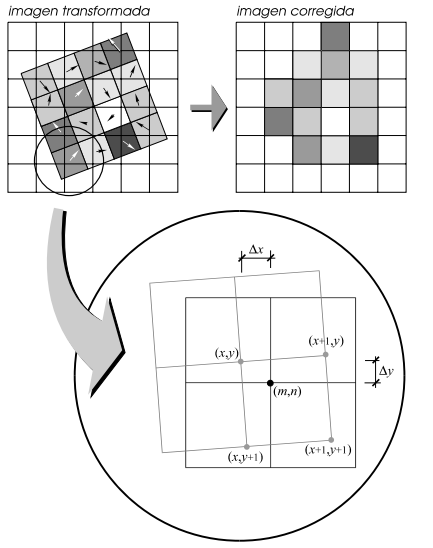
\includegraphics[width=0.6	\textwidth]{./Figures/cap3/vecinoMasCercano2.png}
				    	\caption{Interpolaci\'on Vecino m\'as Cercano.}
				    	\label{fig:vecinoMasCercano2}
				    \end{figure}
		
		\item \textbf{Interpolaci\'on bilineal:} promedia del nivel digital de los cuatros pixeles m\'as cercanos en la imagen original. Este promedio se ponderan seg\'un la distancia del pixel original al corregido; tienen una mayor influencia aquellos pixeles m\'as cercanos en la imagen inicial, pero tienden a difuminar un tanto los contrastes espaciales de la imagen original. Se representa con la siguiente expresi\'on:
		\begin{equation}
		f(x^{,},y^{,}) = c_{1}f(x,y)+c_{2}f(x+1,y)+c_{3}f(x,y+1)+c_{4}f(x+1,y+1)
		\end{equation}	

		\nomenclature[18]{$ c_{j} $}{ Peso asociado a los coeficiente del polinomio bilineal.}
		Donde $ c_{j} $ es un peso asociado a cada valor digital proporcional a la proximidad entre ellos $ (1-\Delta x, 1-\Delta y) $, medida entre los centros de celdas \ref{ec:centros}.
		\begin{equation}\label{ec:centros}
		\begin{cases}
		c_{1} = (1-\Delta x)(1-\Delta y)\\
		c_{2} = \Delta x(1-\Delta y)\\
		c_{3} = (1-\Delta x)\Delta y\\
		c_{4} = \Delta x \Delta y
		\end{cases}
		\end{equation}	
		
		La siguiente ilustraci\'on \ref{fig:bilineal2} nos presenta gr\'aficamente el muestreo bilineal.
		    \begin{figure}[H]
		    	\centering
		    	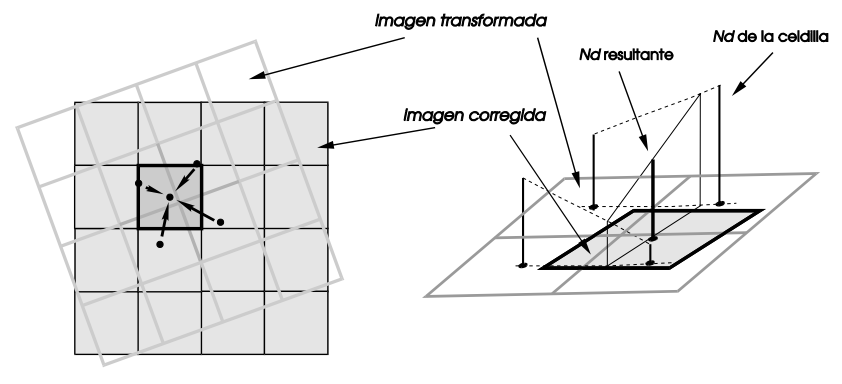
\includegraphics[width=0.9	\textwidth]{./Figures/cap3/bilineal2.png}
		    	\caption{Interpolaci\'on Bilineal.}
		    	\label{fig:bilineal2}
		    \end{figure}
		\item \textbf{Convoluci\'on c\'ubica:} es similar a la interporlaci\'on bilineal pero considera niveles digitales de los 16 pixeles m\'as pr\'oximos. El efecto visual es m\'as correcto, pero supone un volumen de c\'alculo mucho m\'as elevado. Inicialmente, los valores digitales se interpolan linealmente en grupos de cuatro lineas de pixeles cada una para formar cuatro interpolantes:
		
		\begin{equation}
		\resizebox{.9 \textwidth}{!} {$
		f(x^{,}) = [(\Delta x)^{3}-(\Delta x)^{2}]f(x+2,y)-[(\Delta x)^{3}-(\Delta x)^{2}-(\Delta x)]f(x+1,y)+[(\Delta x)^{3}-2(\Delta x)^{2}+1]f(x,y)-[(\Delta x)^{3}-2(\Delta x)^{2}+(\Delta x)]f(x-1,y)
		$}
		\end{equation}	
		Posteriormente se realiza otra interpolaci\'on lineal entre los cuatros valores obtenidos para asignar el resultante a la celda corregida:
		\begin{equation}\resizebox{.9 \textwidth}{!}{$
		f(x^{,},y^{,}) = [(\Delta y)^{3}-(\Delta y)^{2}]f(x^{,}+2)-[(\Delta y)^{3}-(\Delta y)^{2}-(\Delta y]f(x^{,}+1)+[(\Delta y)^{3}-2(\Delta y)^{2}+1]f(x^{,})-[(\Delta y)^{3}-2(\Delta y)^{2}+(\Delta y)]f(x^{,}-1)
		$}
		\end{equation}	
		La siguiente ilustraci\'on \ref{fig:convCubica2} nos muestra graficamente la convoluci\'on c\'ubica:
		
		    \begin{figure}[H]
		    	\centering
		    	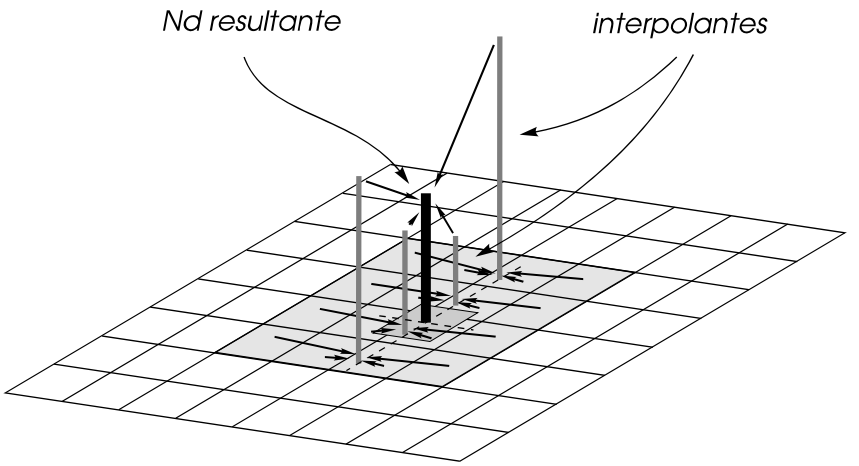
\includegraphics[width=0.9	\textwidth]{./Figures/cap3/convCubica2.png}
		    	\caption{Convoluci\'on c\'ubica.}
		    	\label{fig:convCubica2}
		    \end{figure}
	\end{itemize}


\subsection{Correcci\'on radiom\'etrica}
La correci\'on radiom\'etrica se encarga de minimizar los desajustes producidos en el registro del valor digital en las celdas de la imagen, de hecho en algunos casos las estaciones receptoras llevan a cabo alg\'un tipo de correcci\'on en el momento de recepci\'on de la imagen. La corrección radiom\'etrica implica por una parte la restauraci\'on de lineas o p\'ixeles perdidos y por otra la correcci\'on del bandeado en la imagen \cite{teledUm}.
    \begin{figure}[H]
    	\centering
    	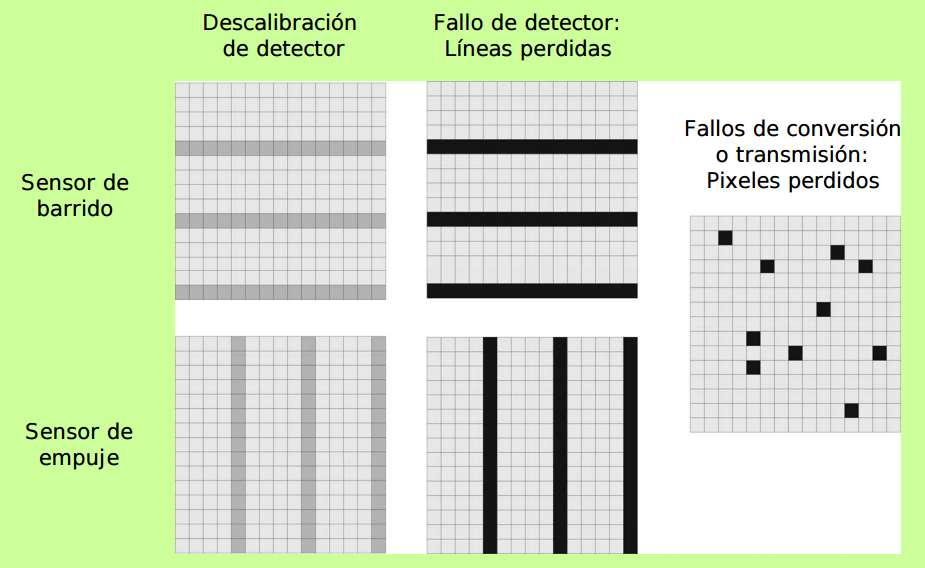
\includegraphics[width=0.9	\textwidth]{./Figures/cap3/correcError.png}
    	\caption{Fallos del sensor en la captura de la imagen.}
    	\label{fig:correcError}
    \end{figure}

\subsubsection{Pixeles o lineas perdidas}\label{subsec:pixelesP}
Si se ha perdido el valor de alg\'un pixel la solución m\'as simple ser\'ia estimarlo como la media de los valores
del mismo pixel en las lineas anterior y posterior (no es recomendable utilizar los pixeles contiguos de la misma linea por que han sido captados por el mismo detector o banda que ha dado el fallo, por tanto son
poco fiables).
		\begin{equation}
		ND_{x,y} = round(\dfrac{ND_{x-1,y} + ND_{x+1,y}}{2})
		\end{equation} 
				\nomenclature[19]{$ ND_{x,y} $}{Nivel digital en la celda $ (x,y) $ de la imagen.}
Siendo $ ND_{x,y} $ el nivel digital en la celda $ (x,y) $ de la imagen, $ round() $ funci\'on que indica el redondeo entero m\'as cercano.\\~\\
Las diferentes bandas ($ k $ y $ r $) de una imagen están altamente correlacionadas y adem\'as los detectores de dos bandas diferentes no son los mismos. Por tanto podría utilizarse el valor del pixel faltante en una banda diferente para mejorar la estimaci\'on:

		\begin{equation}
		ND_{x,y,k} = round((\dfrac{\sigma_{k}}{\sigma_{r}}(ND_{x,y,r}-\dfrac{ND_{x+1,y,r} - ND_{x-1,y,r}}{2}) + \dfrac{ND_{x+1,y,k} + ND_{x-1,y,k}}{2})
		\end{equation} 	
En caso de que la imagen abarque un territorio amplio y cambiante resulta recomendable calcular los coeficientes de correlaci\'on y las desviaciones t\'ipicas ($ \sigma_{k} $ y $ \sigma_{r} $) en un entorno cercano al pixel perdido.\\~\\
Para detectar lineas perdidas se compara la media de los $ ND $ de una linea con las medias de las lineas anterior y posterior, para detectar pixeles perdidos se compara el valor de un pixel con los de los 8 pixeles vecinos mediante alg\'un procedimiento de filtrado.
\subsubsection{Bandeado}\label{subsec:bandeado}
El fen\'omeno del bandeado se debe a una mala calibraci\'on entre detectores y resulta especialmente visible en las zonas de baja radiancia (zonas marinas por ejemplo). El resultado es la aparici\'on peri\'odica de una banda m\'as clara u oscura que las dem\'as.
Para corregir el bandeado se asume que, en caso de no haber error, los histogramas obtenidos por cada uno de los detectores ser\'ian similares entre s\'i y similares al histograma global de la imagen que se toma como referencia.\\~\\
En primer lugar se calculan los coeficientes $ a_{k} $ y $ b_{k} $ para una correcci\'on lineal de cada uno de las bandas.
		\begin{equation}
		b_{k}=\dfrac{\sigma_{r}}{\sigma_{k}}
		\end{equation} 	
				\begin{equation}
				a_{k}=\mu_{r} - b_{k}\mu_{k}
				\end{equation} 	
				
\nomenclature[20]{$ \mu $}{Valor de la media.}
\nomenclature[20]{$ \sigma $}{Desviaci\'on t\'ipica.}
Donde $ \mu $ y $ \sigma $ son la media y la desviaci\'on t\'ipica del conjunto de pixeles de la imagen para los detectores. A continuaci\'on los $ ND $ de la imagen se recalculan como:
				\begin{equation}
				ND_{x,y,k}^{'} = a_{k}+b_{k}ND_{x,y,k}
				\end{equation} 	
asumiendo que la linea $ x $ pertenece a la banda $ k $.				

    \begin{figure}[H]
    	\centering
    	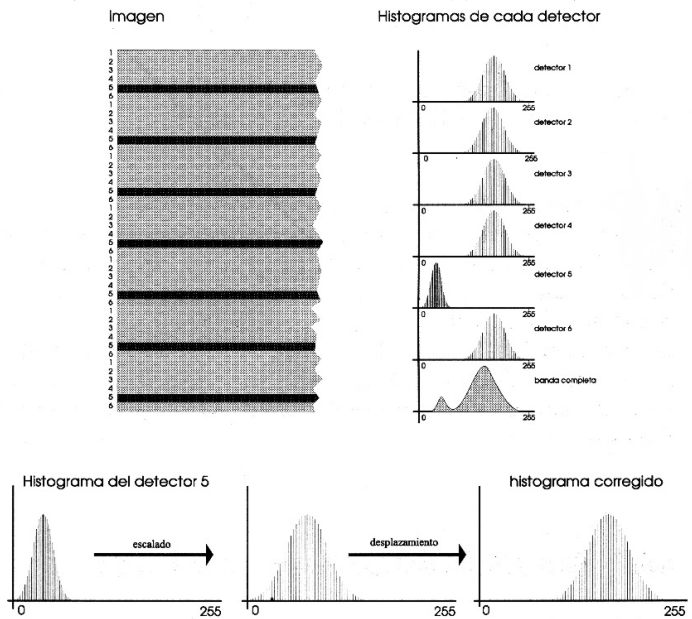
\includegraphics[width=0.9	\textwidth]{./Figures/cap3/bandeo_k.png}
    	\caption{Proceso de correcci\'on del bandeo.}
    	\label{fig:bandeado}
    \end{figure}

\section{Proceso de detecci\'on de cambios}
En los m\'etodos comunes de detecci\'on de cambios se asigna un valor correspondiente al grado de cambio sobre cada celda, independientemente del resto de la imagen. En estos m\'etodos se considera la celda como unidad b\'asica (\'algebra de imagen) para aplicar las correspondientes operaciones matem\'aticas asociadas a cada algoritmo.\\~\\
Los m\'etodos de comparaci\'on, generan una imagen (\'indice de cambios) que representa el grado de cambio entre dos situaciones temporales; las celdas de la imagen resultante, contienen una variable continua de tipo cuantitativo, por lo que se requieren t\'ecnicas que los conviertan en variables cualitativa\cite{martinez2013normalizacion}.
\subsection{Comparaci\'on multitemporal}\label{subsec:compMult}
La comparaci\'on parte de un par de im\'agenes semejantes que abarcan la misma zona de estudio, siguiendo una secuencia multitemporal; cuando los conjuntos de im\'agenes son de car\'acter radiom\'etrico, se recomienda haber aplicado un proceso previo de correcci\'on radiom\'etrica. Singh\cite{singh1989review}, Chuvieco\cite{chuvieco1998factor} y Estornell\cite{estornell2004analisis}, muestran como operaciones más utilizadas:
	\begin{itemize}
		\item \textbf{Diferencia de im\'agenes:} es el m\'etodo m\'as simple, f\'acil de interpretar y directo, ya que consiste en una diferencia algebraica entre los niveles digitales ($ ND $ ) inicial y final para la obtenci\'on de un \'indice ($ I_{dif} $). Normalmente es realizada combinada  con extracciones de \'indices espectrales.
								\begin{equation}
								I_{dif} = ND_{final}-ND_{inicial}
								\end{equation} 	
\nomenclature[21]{$ I_{dif} $}{Indice de cambio por diferencia de im\'agenes.}
\nomenclature[21]{$ I_{ratio} $}{Indice de cambio por el m\'etodo de ratio.}
				\item \textbf{Ratio:} se obtiene aplicando la operación de cociente, entre los niveles digitales ($ ND $ ) inicial y final para la obtenci\'on de un \'indice ($ I_{ratio} $). Podr\'ia  generar mejores resultados pero no se ajusta a una distribución normal.
										\begin{equation}
										I_{ratio} = \dfrac{ND_{final}}{ND_{inicial}}
										\end{equation} 	

		\end{itemize}
Estas dos operaciones generan un \'indice de cambios a partir de cada conjunto de datos multitemporal, dando lugar a tantos mapas de cambios como bandas/capas se consideren; son de gran utilidad cuando se trabaje con im\'agenes pancrom\'aticas o \'indices espectrales/texturales.
\subsection{Criterios de decisi\'on}
La comparaci\'on multitemporal facilita im\'agenes continuas del cambio. En otras palabras, el resultado de los c\'alculos es una imagen en donde el valor de salida indica el grado de cambio, desde la mayor p\'erdida a la mayor ganancia, en una escala gradual. Si se pretende generar una imagen binaria (cambio/estable), es preciso se\~{n}alar un umbral que delimite ambas categor\'ias en las im\'agenes. Ah\'i se plantea un problema de dif\'icil soluci\'on ya que no existen criterios de aplicación general.\\~\\
Si el cambio abarca un sector importante de la imagen, el histograma de la imagen de cambios debiese mostrar un perfil bimodal, lo que permitir\'ia establecer umbrales naturales de cambio, aunque esta situaci\'on no es muy habitual, ya que los cambios en la naturaleza no suelen producirse de modo abrupto\cite{martinez2013normalizacion}.\\~\\
Si es necesario establecer un umbral para separar las \'areas de cambio, puede optarse por se\~{n}alar alg\'un criterio estad\'istico, como la media y la desviaci\'on t\'ipica de una serie de p\'ixeles elegidos aleatoriamente. En ocasiones se ha propuesto utilizar unas \'areas de entrenamiento para calcular que rango de desviaci\'on se pod\'ia considerar l\'imite para p\'ixeles estables, aplicando luego ese valor al conjunto de la imagen\cite{tung1988determination}.

\subsubsection{Discriminaci\'on de las zonas de cambio}\label{sec:discriminacion}
El m\'etodos ($ B(I_{c}) $), de la ecuaci\'on \ref{ec:umbralizacion}, genera una m\'ascara binaria de cambios (0, No Cambio; 1, Cambio) aplicando un umbral ($ U $) especifico sobre la imagen resultante del proceso de comparaci\'on multitemporal \cite{singh1989review}. Son f\'acilmente implementables en procesos de car\'acter autom\'atico/semiautom\'atico. Según Estornell \cite{estornell2004analisis}, partiendo de la hip\'otesis de que el porcentaje de cambios es muy reducido, los valores correspondientes se encuentran situados en los extremos del histograma de frecuencias. Para generar una m\'ascara de cambios es preciso se\~{n}alar un umbral que delimite ambas categorías (cambio/no cambio) a partir del \'indice de cambios ($ I_{c} $)\cite{radke2005image}.	
\begin{equation}\label{ec:umbralizacion}
B(I_{c}) = \begin{cases}
1 & \text{si se cumple que } \abs{I_c} \geq U \\
0 & \text{en cualquier otro caso}
\end{cases}
\end{equation}

\nomenclature[22]{$ I_{c} $}{Indice de cambio.}
\nomenclature[23]{$ B(I_{c}) $}{Funci\'on que genera una mascara de cambio a partir de $ I_{c} $.}
\nomenclature[24]{$ U $}{Umbral de cambio.}

En Rodriguez-Galiano \cite{rodriguez2010analisis} se propone, como criterios de decisi\'on, el m\'etodo de discriminaci\'on basado en los par\'ametros estad\'isticos del \'indice de cambio entre la secuencia temporal de im\'agenes:
\begin{equation}
U=\mu \pm n\sigma
\end{equation}
\nomenclature[24]{$ n $}{Coeficiente de fiabilidad de los datos.}
Donde, el valor de umbral entre cambio/no cambio $ (U) $ se estima en funci\'on de los par\'ametros estad\'isticos $ (\mu, \sigma) $ y un coeficiente de tolerancia $ n $ asignado en base a la fiabilidad de los datos. En Estornell \cite{estornell2004analisis} se clasifican los resultados en funci\'on de $ n $; alta probabilidad de cambio $ (n \geq 2) $ y
zonas de media probabilidad de cambio $ (1 < n < 2) $.

\subsection{Filtrado}
Los filtros constituyen unos de los principales m\'etodos del procesamiento digital de im\'agenes . Pueden usarse para distintos fines, pero siempre, el resultado sobre cada pixel depende de los pixeles en su entorno. Tiene como objetivos: 
	\begin{itemize}
		\item \textbf{Suavizar la imagen:} reducir las variaciones de intensidad entre p\'ixeles vecinos.
		\item \textbf{Eliminar ruido:}  modificar aquellos p\'ixeles cuyo nivel de intensidad es muy diferente al de sus vecinos.
		\item \textbf{Realzar la imagen:} aumentar las variaciones de intensidad, all\'i donde se producen.
		\item \textbf{Detectar bordes::} detectar aquellos p\'ixeles donde se produce un cambio brusco en la funci\'on intensidad.	
	\end{itemize}
\subsubsection{Filtro de la mediana}\label{subsec:filMediana}
El filtrado tiene como ventaja de que el valor final del pixel es un valor real presente en la imagen, siendo dicha variable, la mediana entre los niveles digitales pertenecientes a su vecindad. La mediana es el valor para el cual el 50 \% de todos los p\'ixeles en el histograma son mayores y 50 \% son menores, al contrario de la media \'esta no es influenciada por los valores m\'aximos o m\'inimos\cite{mehl1997fundamentos}.

    \begin{figure}[H]
    	\centering
    	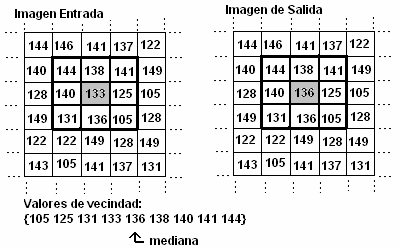
\includegraphics[width=0.8	\textwidth]{./Figures/cap3/FiltrodelaMediana.png}
    	\caption{Proceso del filtro de mediana.}
    	\label{fig:filMediata}
    \end{figure}

\section{Resumen}

La utilizaci\'on de im\'agenes satelitales implica un pre-procesamiento adicional, diferente a las que se le realiza a im\'agenes normales. Estos pre-procesamientos van ligados a resoluciones, firmas espectrales y tipos de im\'agenes satelitales propias del sensor espacial que captura la informaci\'on. En este capitulo se brinda conceptos relacionados a lo descripto en lo anterior, como tambi\'en se describen conocimientos previos para aplicar an\'alisis multitemporales y detecci\'on de cambio en im\'agenes de sat\'elite que componen piezas fundamentales en la metodolog\'ia propuesta.